% =============================================================================
% DSR PROFILE MANUSCRIPT DELTA
% =============================================================================
% This file is NOT a second full paper. It is a replacement-ready delta
% against qward/examples/papers/main.tex: only the title, abstract, keywords,
% and the specific paragraphs/equations/tables/figures that must change to
% reflect the DSR evaluation *profile* (Success Rate, Chance-Corrected
% Success, Coarse TVD Similarity, Coarse Hellinger Fidelity, with the
% original Michelson-contrast DSR demoted to an optional fifth "peak-contrast"
% layer) are included below, each block labeled with the main.tex location
% it replaces. Everything not listed here (Background, most of Related Work,
% Execution model, most of Discussion structure) is UNCHANGED.
%
% Underlying data: DSR_result.csv rebuilt via
%   PYTHONPATH=. uv run python qward/examples/papers/enrich_dsr_profile.py --dataset all
%   PYTHONPATH=. uv run python qward/examples/papers/build_csv_from_json.py
% 1,283 rows total (248 Grover, 239 QFT, 796 Teleportation) -- the row count
% differs slightly from the original paper's 1,281 (246 Grover, 239 QFT, 796
% Teleportation): QFT and Teleportation counts are unchanged, and Grover
% gained 2 rows (S2-1 on ibm_fez, optimization levels 2 and 3) that come
% from a raw result file (S2-1_IBM_ibm_fez_20260617_105053.json) added to
% the dataset after the original submission, unrelated to the DSR-profile
% recomputation itself. See the reproducibility checklist at the end of
% this file.
% =============================================================================


% =============================================================================
% BLOCK 1 -- REPLACES main.tex lines 64, 109-119 (title, abstract, keywords)
% =============================================================================

\title{DSR: A Lightweight Evaluation Profile for Known-Answer Quantum Tasks}

\begin{abstract}

Validating program correctness is a fundamental requirement in software engineering. In classical computing, the deterministic nature of execution enables direct validation by comparing an observed output against an expected value. In contrast, quantum computing (QC) is inherently stochastic: the outcome of an execution is a probability distribution, and validation traditionally requires simulating the full ideal distribution and comparing it against the observed histogram --- a step whose cost grows exponentially with the number of qubits and becomes infeasible for circuits beyond the classical simulation wall. This paper presents the \emph{Differential Success Rate (DSR) evaluation profile}, a histogram-free evaluation methodology for quantum jobs whose correct answers form a small, analytically known set~$E$ (e.g., the marked states in Grover's search, the input state of a QFT round-trip, or a teleportation payload). From only the observed counts and~$E$, the profile reports four complementary, per-job components --- \emph{Success Rate}, \emph{Chance-Corrected Success}, \emph{Coarse TVD Similarity}, and \emph{Coarse Hellinger Fidelity} --- computed without ever constructing the $2^n$-outcome ideal distribution. The original Michelson-contrast score from our earlier formulation is retained as an optional fifth \emph{peak-contrast} layer, motivated by a documented failure mode in which it collapses to zero under amplitude-damping noise even when the profile's other components still separate providers clearly.

We recompute the profile on 1{,}283 jobs spanning Grover's search (248), the Quantum Fourier Transform (239), and a variation of the teleportation protocol (796), executed on multiple QPUs from IBM Quantum and Rigetti via AWS, and add a new broad-ideal experiment (multi-marked Grover up to 40 qubits) to demonstrate the profile's histogram-free advantage at scales where the exact ideal distribution cannot be computed on any classical machine. The profile confirms that Rigetti's Ankaa-3/Forte-1 devices degrade earlier than IBM's Heron~R2 processors on Grover and QFT (e.g., chance-corrected success at 3~qubits: IBM median~$0.78$ vs.\ Rigetti~$0.00$, Cliff's~$\delta=+1.00$), and reveals a new, previously invisible result for teleportation: at payload sizes~3--4, IBM's chance-corrected success is essentially zero ($\leq 0.01$) while Rigetti's remains substantially above chance ($0.15$--$0.31$, $p<0.0001$), even though the legacy Michelson score collapses to~$0$ on both providers --- direct evidence for the profile's motivating T1-bias failure mode. These findings position the DSR profile as a lightweight, task-level complement to full-distribution fidelity metrics, applicable specifically to known-answer workloads and scalable to problem sizes where those metrics are not computable at all.

\end{abstract}

\begin{IEEEkeywords}
Differential success rate, quantum output validation, histogram-free evaluation, chance-corrected success, probability distribution analysis, fidelity metrics, NISQ benchmarking, quantum software testing, Hellinger fidelity, total variation distance, IBM Quantum, Rigetti
\end{IEEEkeywords}


% =============================================================================
% BLOCK 2 -- REPLACES main.tex lines 133, 137 (Introduction, novelty framing)
% =============================================================================
% Keep paragraphs at lines 121-131 and 134-136 UNCHANGED. Replace only the
% paragraph at line 133 (the one introducing DSR) and line 137 (the summary
% of experimental contributions), to frame the contribution as an evaluation
% *methodology* rather than a new algebraic score, and to add the new
% broad-ideal experiment and teleportation finding to the roadmap.

In this paper, we introduce the \emph{DSR evaluation profile}, a task-level, histogram-free evaluation methodology for quantum jobs whose correct answers form a known set~$E$. Rather than proposing a single new scalar formula, the profile packages four complementary, "higher-is-better" components --- Success Rate, Chance-Corrected Success, Coarse TVD Similarity, and Coarse Hellinger Fidelity --- each computed directly from measurement counts and~$E$, without simulating the ideal distribution over all $2^n$ outcomes. This lineage connects DSR to chance-corrected agreement statistics used elsewhere for imbalanced or above-random-guessing evaluation (e.g., Cohen's~$\kappa$-style correction) and to randomized-benchmarking-style polarization, adapted here to the single-job, known-answer setting. The original Michelson-contrast formulation from our earlier work is retained as an optional fifth "peak-contrast" layer, since it captures a distinct quantity (dominance over the strongest \emph{competing} peak, rather than over chance) and has documented value as a motivating counter-example (Section~\ref{sec:dsr}).

Our experiments demonstrate the usefulness of the DSR profile for improving the interpretability of quantum jobs across the Grover and QFT algorithms on two quantum providers, and for a teleportation variant, by correlating each profile component with the number of qubits, circuit depth, and provider. We further design a broad-ideal, known-answer experiment (multi-marked Grover up to 40~qubits) to demonstrate that the profile remains computable exactly where full-distribution fidelity metrics are not: at 14~qubits, computing the ideal statevector and the resulting Hellinger fidelity/TVD already takes over a minute locally, while the histogram-free profile computes in under a millisecond regardless of qubit count, and beyond roughly 30~qubits the ideal-distribution comparison is not just slow but requires more memory than exists on any single machine. In addition, we empirically compare the profile against Hellinger fidelity (HF) and TVD fidelity (TVDF), showing where the four components agree, where they diverge for multi-answer tasks, and where recomputing the empirical narrative from our earlier Michelson-only analysis surfaces a previously invisible provider-dependent effect in teleportation.


% =============================================================================
% BLOCK 3 -- INSERTS after main.tex line 186 (end of Section III, Related Work)
% =============================================================================
% New subsection addressing Reviewer 1's point that HF/TVDF remain applicable
% via inverse-circuit ("uncompute to zero") constructions even without a
% known target set, and explaining why the DSR profile is not a competing
% general-purpose replacement for that use case.

\subsection{Inverse-Circuit Fidelity as a General-Purpose Alternative}
\label{sec:inverse-circuit}

HF and TVDF are not restricted to algorithms with a known target set: given any circuit~$U$, one can append its inverse~$U^\dagger$ and measure the deviation of the resulting counts from the all-zero state, obtaining a task-agnostic fidelity proxy applicable to essentially any circuit, including variational algorithms with no analytically known output. This generality is a genuine advantage of HF/TVDF over the DSR profile, which requires a known~$E$ and therefore cannot be applied to circuits with no verifiable target. However, the inverse-circuit construction doubles circuit depth, which compounds hardware noise and biases the resulting fidelity downward relative to a direct histogram comparison at the same qubit count; it also concentrates the "success" outcome on a single zero-heavy bit string, which is precisely the target profile (single, all-zero-biased~$E$) that the T1-bias motivation in Section~\ref{sec:dsr} identifies as failure-prone for the peak-contrast (Michelson) layer specifically, though not for the chance-corrected and coarse-similarity components. We therefore do not position the DSR profile as competing with inverse-circuit HF/TVDF for target-agnostic validation; the profile is scoped to workloads (search, transform, and state-preparation/transmission tasks) where a task-native~$E$ is already known without needing to construct an inverse circuit, and where the histogram-free property lets the evaluation scale past the qubit counts at which any full-distribution comparison --- inverse-circuit or otherwise --- becomes intractable (Section~\ref{sec:broad-ideal}).


% =============================================================================
% BLOCK 4 -- REPLACES main.tex lines 201-310 (Section V, "Differential Success
% Rate" -> "DSR Evaluation Profile")
%
% IMPORTANT for whoever applies this delta: the equations, table, and figure
% originally defined in this range (Eq.~p_x, p_exp, p_exp_bar, p_comp, dsr
% [Michelson], dsr_ratio, dsr_log, dsr_nm; Table~tab:dsr_variants;
% Figure~fig:dsr_variants) are NOT deleted. Eq.~p_x and p_exp are kept
% in place (p_exp is simply renamed "Success Rate" and reused as $p_E$
% below, same label, same equation, no redefinition). Eq.~p_exp_bar,
% p_comp, dsr, dsr_ratio, dsr_log, dsr_nm, Table~tab:dsr_variants, and
% Figure~fig:dsr_variants are RELOCATED (physically moved, not rewritten)
% into the new "Optional fifth layer" subsection at the end of this block,
% where they are cited by their original labels via \eqref/\ref exactly as
% before -- do not duplicate-define them elsewhere in the merged document.
% =============================================================================

\section{DSR Evaluation Profile}
\label{sec:dsr}

The DSR evaluation \emph{profile} is a per-job result consisting of four histogram-free, task-level components, computed only from measurement counts and an analytically known expected-outcome set~$E$ (size $K=|E|$). None of the four components requires simulating the ideal distribution over all $2^n$ outcomes. We use \emph{evaluation profile} rather than \emph{score} or \emph{metric} deliberately: the four components answer different questions and are reported separately rather than averaged, and (as detailed below) only two of the four are metrics in the strict mathematical sense.

Although the profile eliminates the need for computationally expensive simulations of the ideal probability distribution, it inherits the same scope restriction as our earlier Michelson formulation: applicability is limited to problems for which the target set~$E$ is known, and none of the four components captures phase-related errors, since all are computed from measurement counts alone.

\subsection{Definitions}

Let $\mathcal{C} : \{0,1\}^m \to \mathbb{Z}_{\geq 0}$ denote the histogram returned by a quantum job over the $m$ \emph{measured} qubits (after any ancilla marginalization), mapping each $m$-bit string $x$ to its observation count $\mathcal{C}(x)$. The total number of shots is $S = \sum_{x} \mathcal{C}(x)$, and the probability of each outcome is estimated as $p_x = \mathcal{C}(x)/S$ (Equation~\eqref{eq:p_x}, unchanged).

Let $E \subseteq \{0,1\}^m$ denote the set of expected outcomes (e.g., the marked states in Grover's algorithm) with $K = |E|$, exactly as originally defined. The profile requires a \emph{task reference distribution} $q : E \to [0,1]$ with $\sum_{x \in E} q(x) = 1$, representing the relative weight each expected outcome \emph{should} carry in an ideal execution. We default to uniform weights $q(x) = 1/K$ only when the task genuinely expects equal weight (e.g., multi-marked Grover, where every marked state is amplified identically). For QFT period detection, the peak weights across~$E$ are in general \textbf{non-uniform} (they follow the analytic $\mathrm{sinc}^2$ envelope of the transform whenever the period does not evenly divide $2^m$); supplying the exact analytic weights is required in that regime, and defaulting to uniform would bias the coarse components below. In our recomputed dataset, every QFT period-detection configuration has a period dividing $2^m$ evenly, so the peaks are exactly uniform and the default applies without bias; we flag this condition explicitly in the enrichment pipeline (\texttt{enrich\_dsr\_profile.py}) rather than assuming it silently.

\subsection{Success Rate and Chance-Corrected Success}

The \emph{Success Rate} is the same quantity originally defined as $p_{\text{exp}}$ (Equation~\eqref{eq:p_exp}, kept as-is, not redefined): the total probability mass on the expected outcomes, $p_E \equiv p_{\text{exp}} = \sum_{x \in E} p_x$. We rename it Success Rate here because, unlike in the original Michelson formulation, it is now reported directly as a profile component rather than only as an intermediate quantity.

Success Rate alone does not indicate whether an observed value is better than random guessing, particularly for small $K$ relative to $2^m$. We define the \emph{chance baseline} as the probability of landing in~$E$ under a uniform random guess over all $2^m$ outcomes, $b = K/2^m$, and the \emph{Chance-Corrected Success} as:

\begin{equation}
\label{eq:profile_chance_corrected}
    \tilde{p}_E = \mathrm{clip}\!\left(\frac{p_E - b}{1 - b},\; 0,\; 1\right)
\end{equation}

so that $\tilde{p}_E = 0$ when the job performs no better than chance and $\tilde{p}_E = 1$ for perfect success, regardless of $K$ or~$m$. Both $p_E$ and $\tilde{p}_E$ are \emph{scores}, not metrics in the formal mathematical sense (they are not distances on a space of distributions).

\subsection{Coarse TVD Similarity and Coarse Hellinger Fidelity}

To capture distributional agreement without the cost of a full $2^m$-outcome comparison, we define a coarse, $(K{+}1)$-bin distribution: one bin per element of $E$, plus a single aggregate \texttt{other} bin for every outcome outside~$E$. The observed coarse distribution is $P_{\text{coarse}} = (p_{x_1}, \ldots, p_{x_K}, p_{\text{other}})$ with $p_{\text{other}} = 1 - p_E$; the reference coarse distribution is $Q_{\text{coarse}} = (q(x_1), \ldots, q(x_K), 0)$, i.e., the task reference weights over $E$ with an ideal \texttt{other} mass of zero. We then report:

\begin{equation}
\label{eq:profile_coarse_tvd}
    \mathrm{TVD}_{\text{coarse}} = \tfrac{1}{2}\sum_{i} \left| P_{\text{coarse}, i} - Q_{\text{coarse}, i} \right|, \qquad
    \mathrm{TVDSim} = 1 - \mathrm{TVD}_{\text{coarse}}
\end{equation}

\begin{equation}
\label{eq:profile_coarse_hf}
    \mathrm{HF}_{\text{coarse}} = \left( \sum_i \sqrt{P_{\text{coarse}, i}\, Q_{\text{coarse}, i}} \right)^2
\end{equation}

$\mathrm{TVD}_{\text{coarse}}$ and the Hellinger \emph{distance} $\sqrt{1-\sqrt{\mathrm{HF}_{\text{coarse}}}}$ are genuine mathematical metrics on the coarse distribution; the reported "higher-is-better" complements, $\mathrm{TVDSim}$ and $\mathrm{HF}_{\text{coarse}}$, are therefore scores, like $p_E$ and $\tilde{p}_E$, not metrics in the strict sense, despite being derived from one.

\subsection{The $K=1$ collapse, precisely scoped}

When $K=1$, the coarse distribution has only two bins (the single expected outcome and \texttt{other}), and by construction $\mathrm{TVDSim} = \mathrm{HF}_{\text{coarse}} = p_E$ \emph{exactly} --- a direct algebraic consequence of Equations~\eqref{eq:profile_coarse_tvd}--\eqref{eq:profile_coarse_hf} at $K=1$, verified numerically to floating-point precision on every $K=1$ row of our recomputed dataset (single-marked Grover, QFT round-trip, and all 796 teleportation jobs). This means the coarse components add no new distributional information beyond Success Rate for $K=1$ tasks; they are informative specifically for $K>1$ tasks (Figure~\ref{fig:multi_answer_divergence}, Section~\ref{sec:metric_comparison}).

This collapse is a property of the coarse profile's \emph{own} construction --- an idealized "succeed on $E$, fail otherwise" target --- and is distinct from asking whether the coarse profile matches the \emph{full}-distribution HF/TVDF computed against a statevector-simulated ideal. The two coincide only when the true ideal probability is itself exactly a delta on $E$: this holds for QFT round-trip and for our teleportation protocol (both deterministic unitaries with a single correct output), but not for finite-iteration Grover, whose true ideal state retains residual amplitude on unmarked states even at the optimal iteration count. Section~\ref{sec:metric_comparison} reports this deviation directly (Figure~\ref{fig:full_vs_coarse}): QFT round-trip points fall exactly on the full-vs-coarse identity line, while Grover deviates by up to $0.23$ in Hellinger fidelity and $0.05$ in TVD fidelity at high success rates.

\subsection{Optional fifth layer: peak-contrast (Michelson) DSR}
\label{sec:michelson-layer}

This subsection relocates, without rewriting, the original definitions of $\bar{p}_{\text{exp}} = p_E/K$ and $p_{\text{comp}} = \max_{x \notin E} p_x$ (Equations~\eqref{eq:p_exp_bar}--\eqref{eq:p_comp}), the Michelson-contrast formulation $\mathrm{DSR}$ (Equation~\eqref{eq:dsr}), and the alternative-formulation study (Table~\ref{tab:dsr_variants}, Equations~\eqref{eq:dsr_ratio}--\eqref{eq:dsr_nm}, Figure~\ref{fig:dsr_variants}), together with all of their originally stated edge-case handling ($S=0$, empty $E$, empty competing set). They are retained as an optional fifth \emph{peak-contrast} layer, distinct from the four profile components above because it contrasts against the strongest competitor rather than the chance baseline. We no longer treat it as the headline result, for two reasons made concrete by the recomputed data.

First, comparing $p_{\text{comp}}$ (a single competing peak) against the chance baseline $b$ (spread uniformly over $2^m - K$ outcomes) means Michelson DSR is sensitive to whichever single outcome happens to concentrate the "failure" mass, while chance-corrected success is not. Second, and more importantly, this creates a specific, previously undocumented failure mode under amplitude damping (T1 relaxation): when a circuit's noise process biases outcomes toward the all-zero state, the competing peak $p_{\text{comp}}$ itself grows toward the same magnitude as $\bar{p}_{\text{exp}}$ (if $E$ is zero-heavy) or dominates it entirely, driving Michelson DSR to exactly zero. We observe this directly in our teleportation data: at payload sizes 2 and 4, the median Michelson DSR is $0.000$ on \emph{both} IBM and Rigetti, even though chance-corrected success clearly separates the two providers at the same payload sizes (IBM $\leq 0.01$ vs.\ Rigetti $0.15$--$0.31$, Section~\ref{sec:metric_comparison}). Michelson DSR alone would report "complete failure, no provider difference" in exactly the setting where chance-corrected success reveals a large, statistically significant gap. This observation is the motivating counter-example for keeping chance-corrected success rather than peak-contrast as the profile's headline component, while still reporting the peak-contrast layer where it adds information (e.g., distinguishing a job that fails toward its own competing structure from one that fails toward pure noise).

Among the four relocated alternative formulations, Michelson remains the selected peak-contrast formulation for the reasons given in the original analysis (widest dynamic range, earliest sensitivity to degradation); nothing in the original selection rationale changes, only its status as an optional rather than headline layer.


% =============================================================================
% BLOCK 5 -- INSERTS a new subsection after main.tex line 382 (end of
% "Workloads" subsection, before "Backends and execution")
% =============================================================================

\subsection{Broad-ideal, known-answer scaling experiment}
\label{sec:broad-ideal}

To directly test the claim that the profile remains usable where full-distribution comparison is not, we add a multi-marked Grover experiment ($K=3$ marked states, fixed) at increasing qubit count~$n$, in two stages. In the first stage ($n \in \{6, 8, 10, 12, 14\}$), we run the real circuit locally via the Qiskit AER simulator and compute \emph{both} the full-distribution path (exact ideal statevector over all $2^n$ outcomes, then Hellinger fidelity/TVD against the observed counts) and the histogram-free profile on the same counts, as a timing comparison and a correctness cross-check. In the second stage ($n \in \{26, 28, 30, 32, 36, 40\}$), no circuit is simulated at all: at this scale, a Grover circuit's ideal statevector requires between 537~MB ($n=26$) and 8.8~TB ($n=40$) merely to store the outcome probabilities, well beyond any single machine's memory; we instead generate representative counts directly (a multinomial sample over the $K$ marked states plus a small set of random \texttt{other} outcomes) as a stand-in for real QPU output, and compute the profile from those counts and the known~$E$ alone.


% =============================================================================
% BLOCK 6a -- REPLACES main.tex line 395 (Results section lead paragraph,
% job counts only; keep the \section{Results}\label{sec:results} heading and
% the rest of the paragraph's framing sentences unchanged)
% =============================================================================

This section presents the empirical results of 1{,}283 QPU runs covering jobs based on the Grover, QFT, and vTP algorithms (248, 239, and 796 jobs, respectively; two additional 2-qubit Grover runs on \textit{ibm\_fez}, added to the dataset after the original submission, account for the difference from 1{,}281). When comparing IBM and Rigetti results side by side (Sections~\ref{subsec:dsr_qubits}, \ref{sec:metric_comparison}), IBM Grover and QFT data are filtered to optimization level~3 to enable a fair comparison with Rigetti, which does not expose optimization levels. The depth analysis (Section~\ref{subsec:dsr_depth}) uses all optimization levels, and the effect of the optimization level is analyzed separately in Section~\ref{subsec:opt_level}. Our analysis covers the degradation of each DSR profile component as a function of qubit count scaling and circuit depth. We also benchmark the profile against full-distribution HF and TVDF to highlight where their behaviors agree and where they diverge.


% =============================================================================
% BLOCK 6 -- REPLACES main.tex lines 397-465 (Sections "DSR versus number of
% qubits", "DSR versus depth", "Effect of optimization level on QFT")
% =============================================================================

\subsection{Profile versus number of qubits}
\label{subsec:dsr_qubits}

Figures~\ref{fig:grover_profile_ibm}--\ref{fig:qft_profile_aws} show the distribution of all four profile components as a function of qubit count, separately for Grover and QFT, on IBM and Rigetti Ankaa-3/Forte-1 backends.

\begin{figure}[ht!]
  \centering
  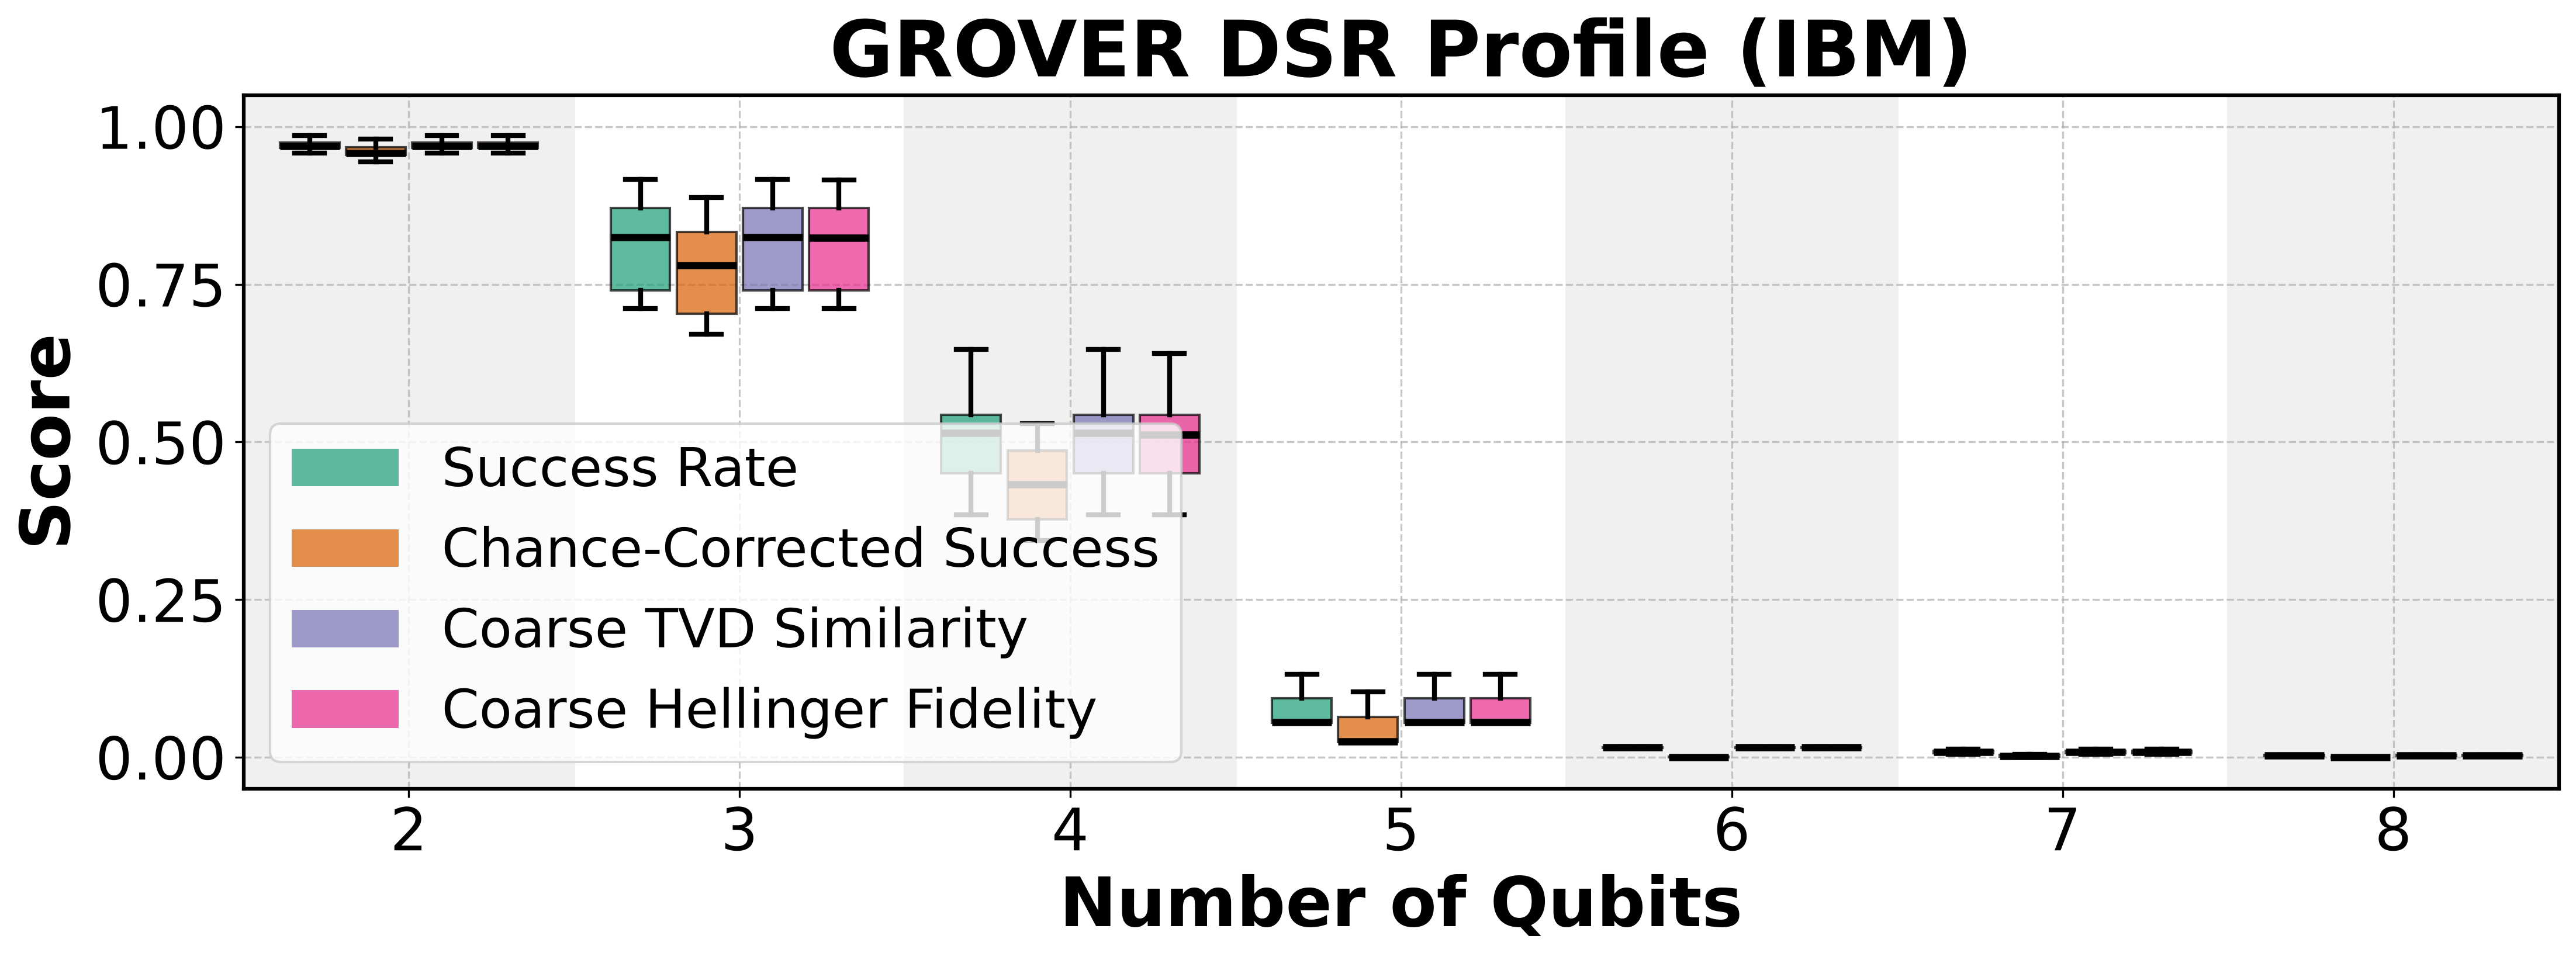
\includegraphics[width=\columnwidth]{plots/2_grover_dsr_profile_comparison_ibm.png}
  \caption{DSR profile (Success Rate, Chance-Corrected Success, Coarse TVD Similarity, Coarse Hellinger Fidelity) for Grover's algorithm vs.\ number of qubits (IBM backends, optimization level~3).}
  \label{fig:grover_profile_ibm}
\end{figure}

\begin{figure}[ht!]
  \centering
  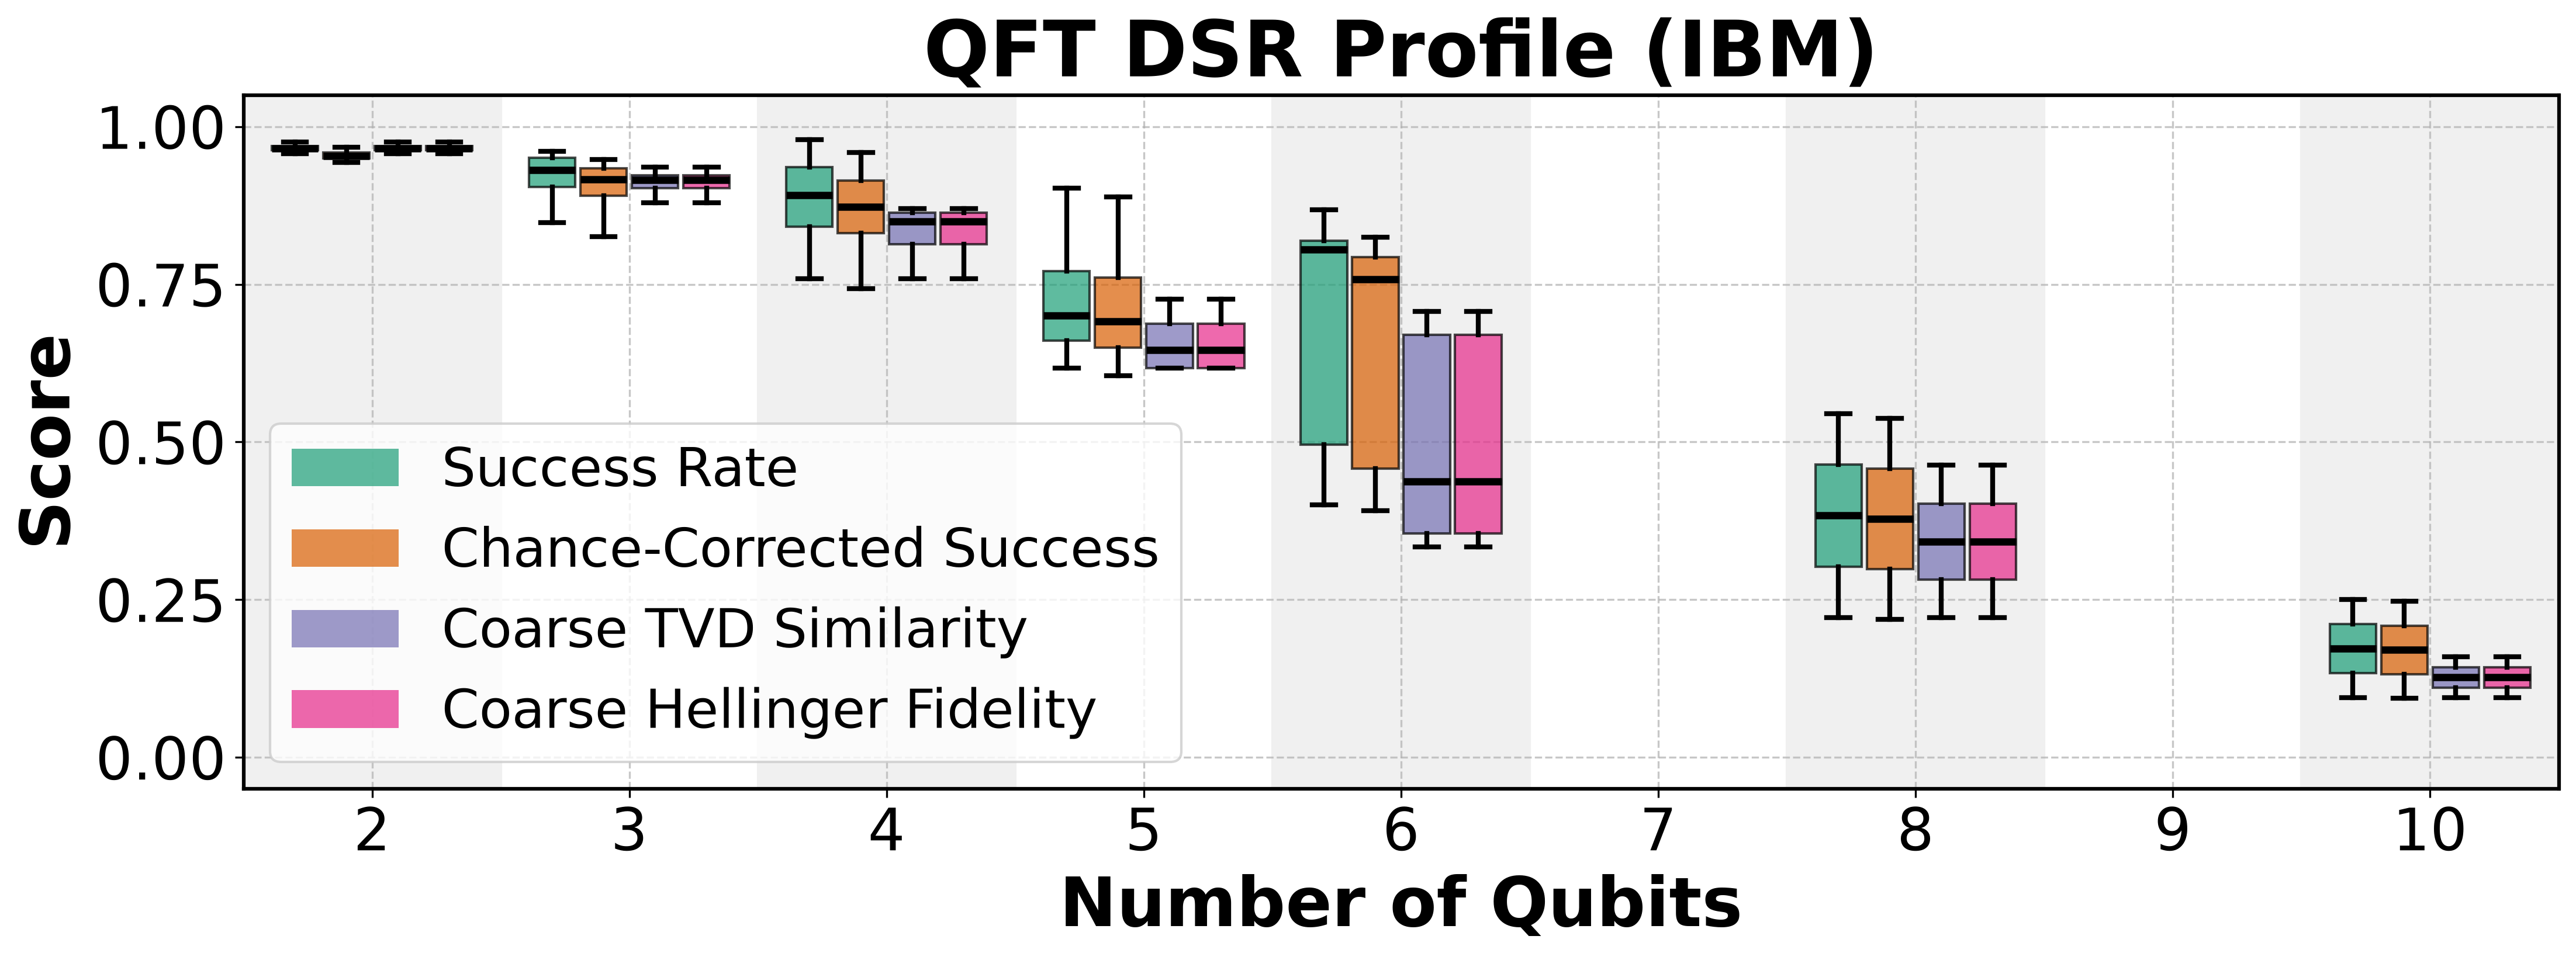
\includegraphics[width=\columnwidth]{plots/2_qft_dsr_profile_comparison_ibm.png}
  \caption{DSR profile for QFT vs.\ number of qubits (IBM backends, optimization level~3).}
  \label{fig:qft_profile_ibm}
\end{figure}

\begin{figure}[ht!]
  \centering
  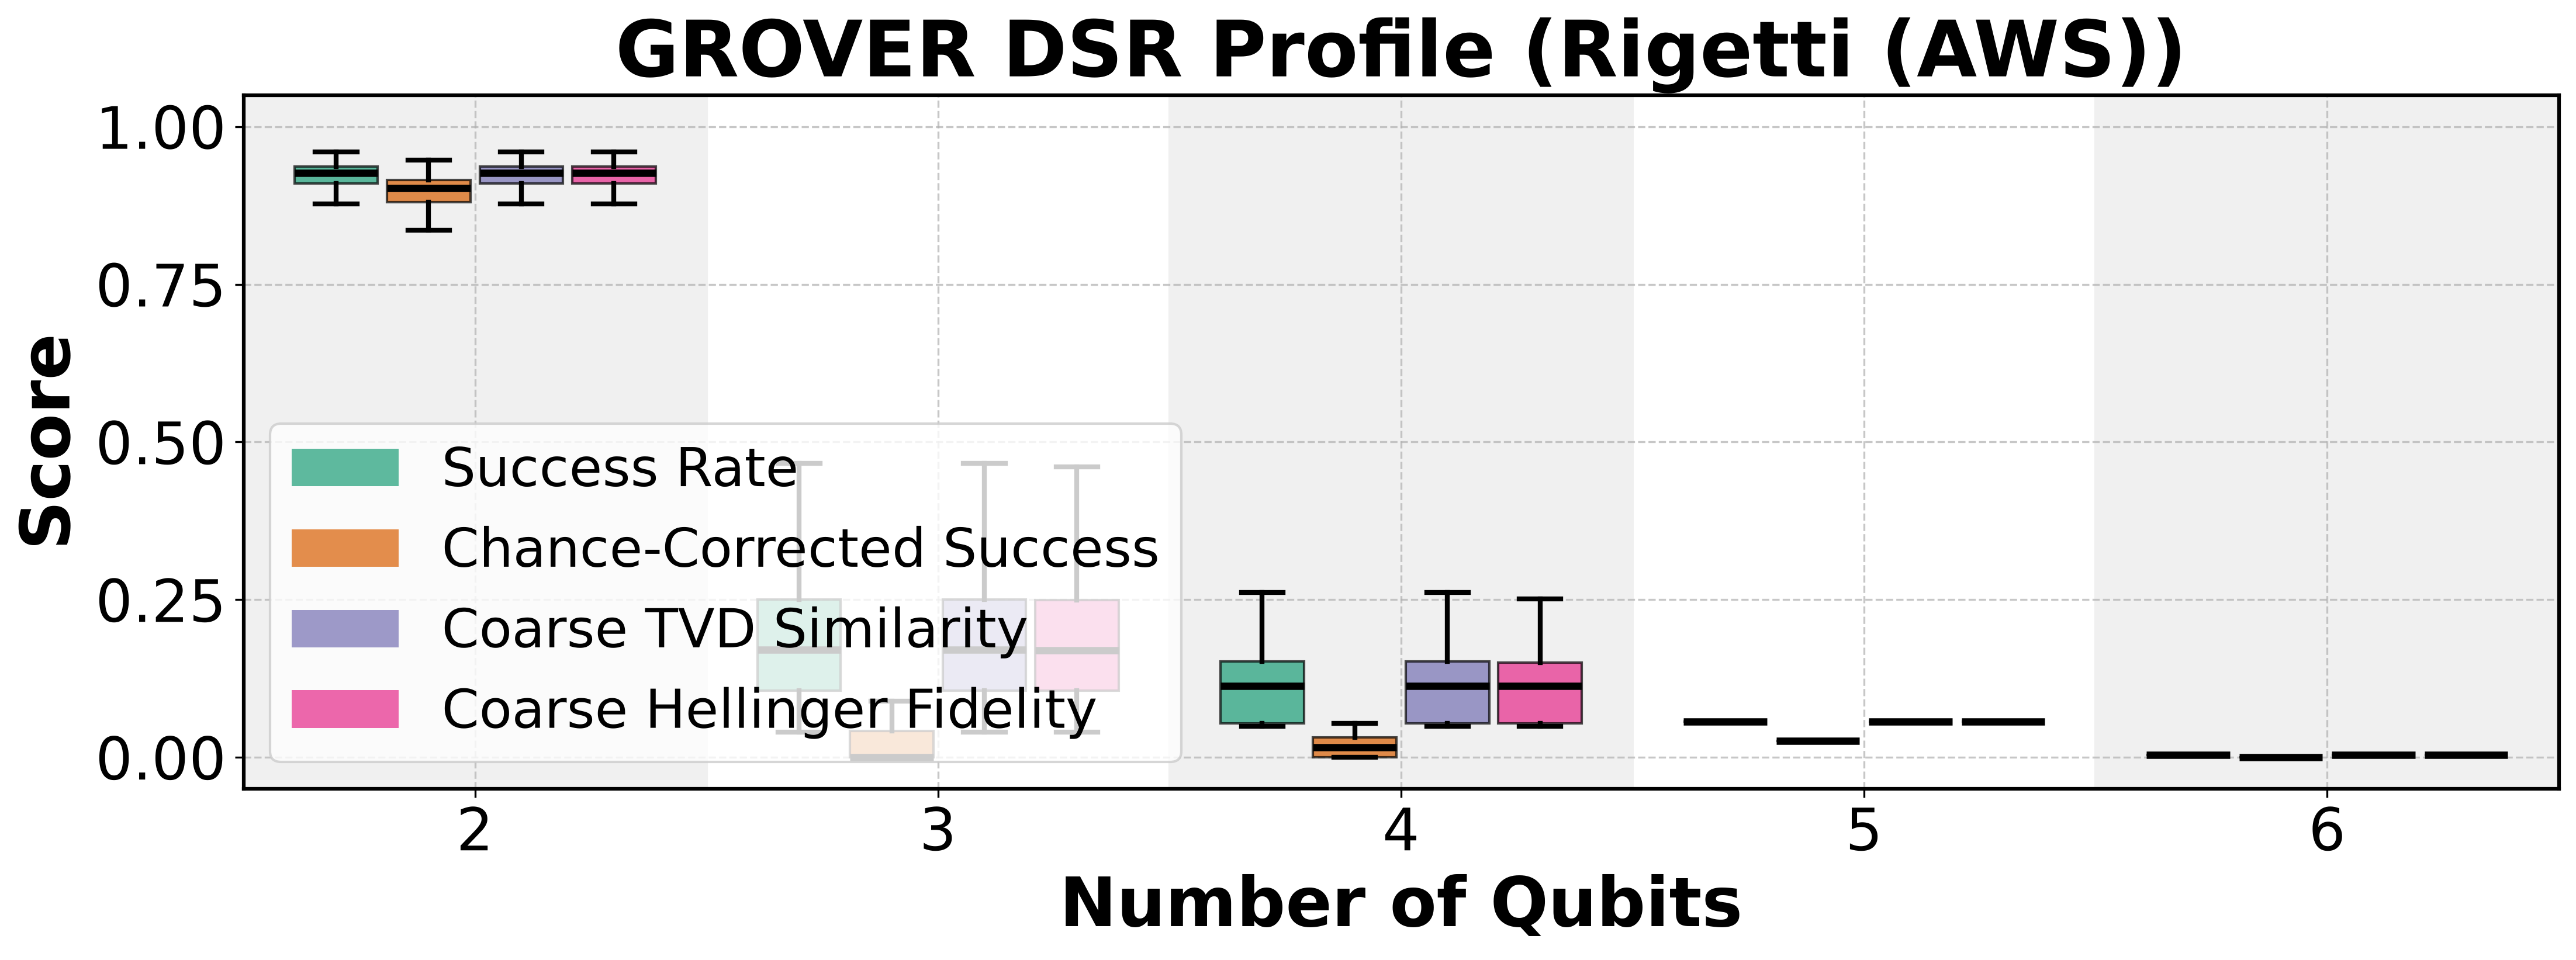
\includegraphics[width=\columnwidth]{plots/2_grover_dsr_profile_comparison_aws.png}
  \caption{DSR profile for Grover's algorithm vs.\ number of qubits (Rigetti Ankaa-3/Forte-1 via AWS).}
  \label{fig:grover_profile_aws}
\end{figure}

\begin{figure}[ht!]
  \centering
  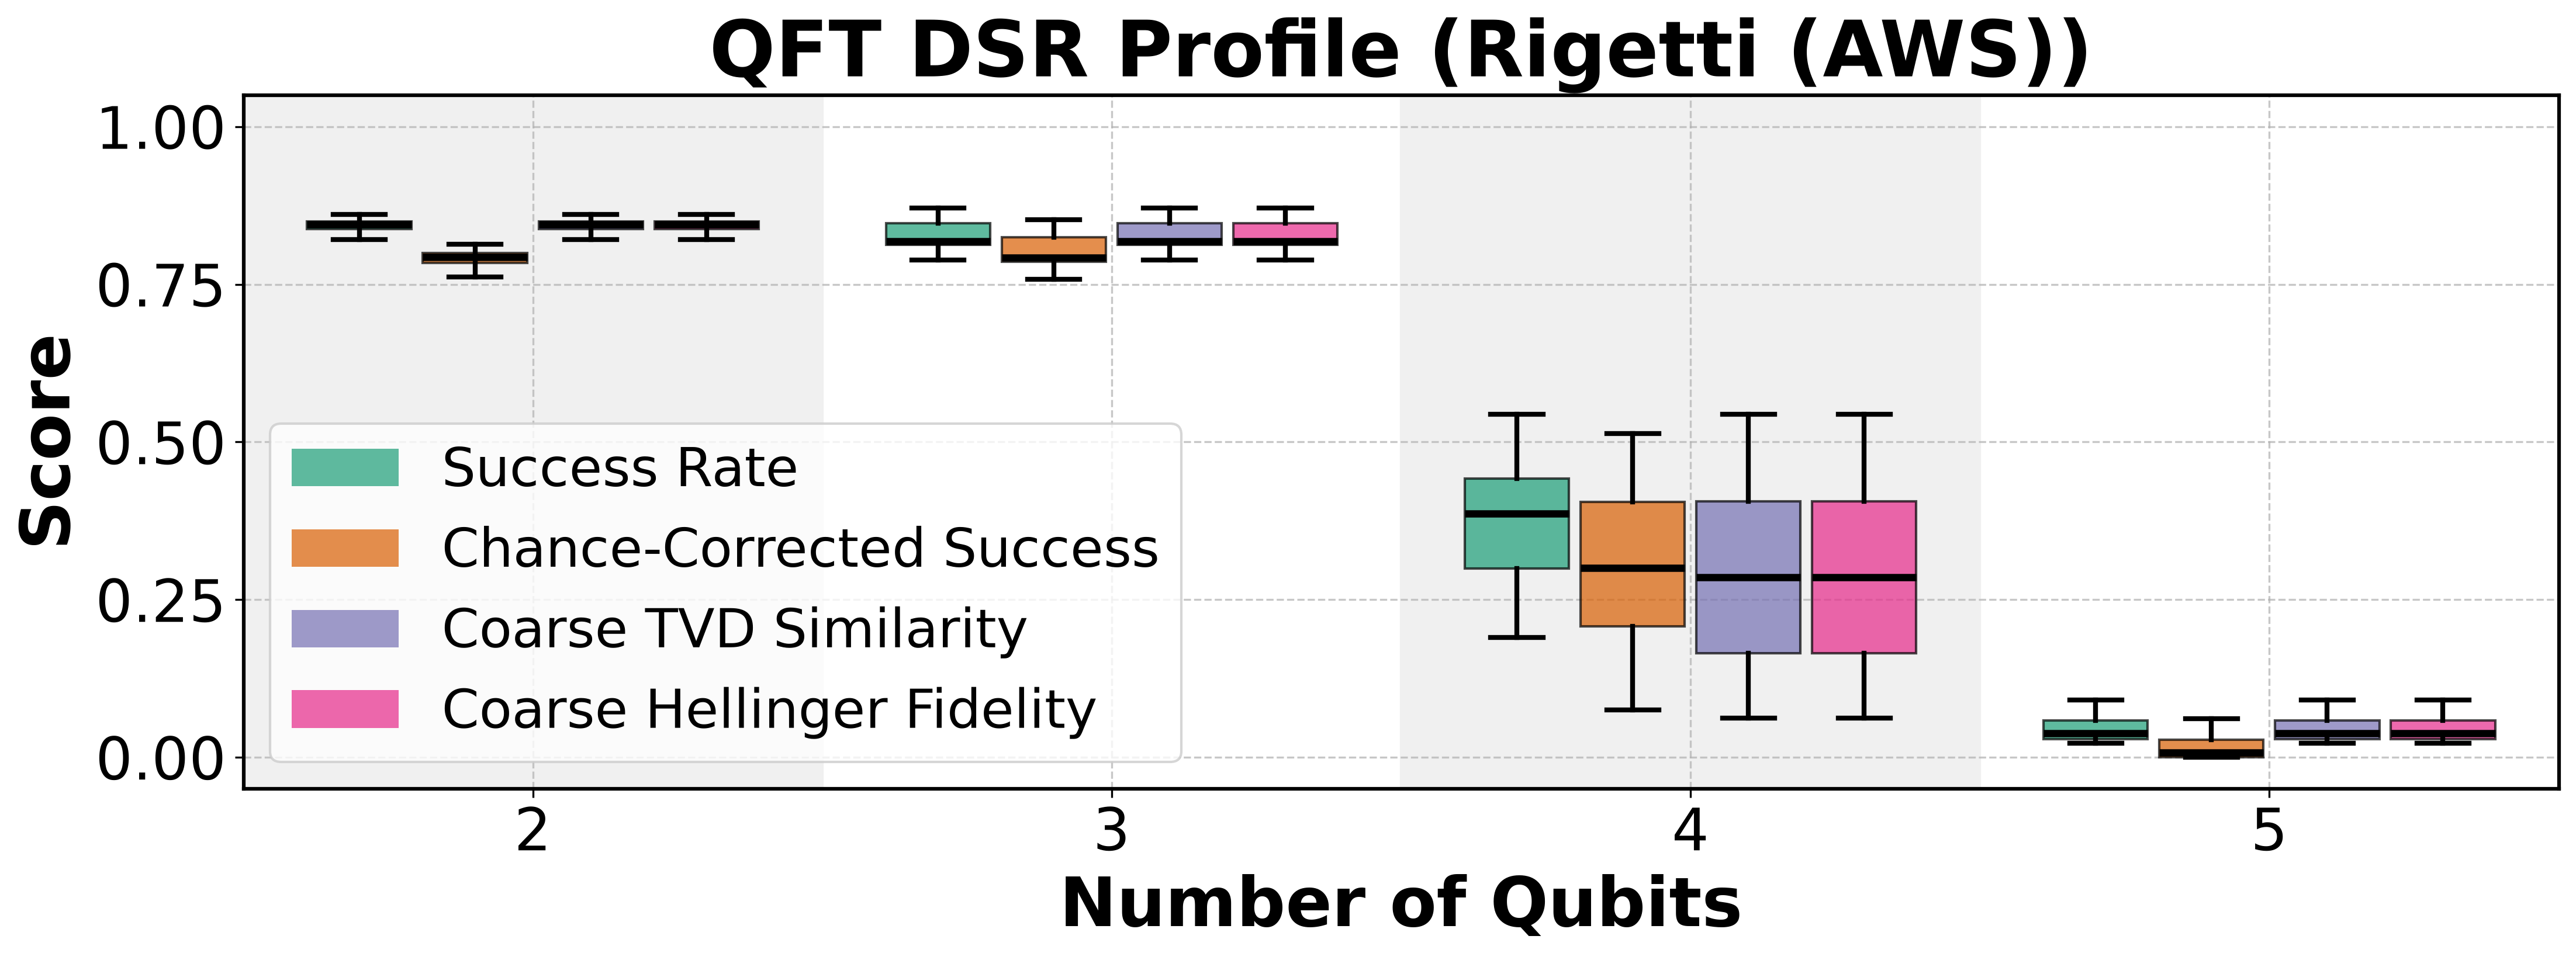
\includegraphics[width=\columnwidth]{plots/2_qft_dsr_profile_comparison_aws.png}
  \caption{DSR profile for QFT vs.\ number of qubits (Rigetti Ankaa-3/Forte-1 via AWS).}
  \label{fig:qft_profile_aws}
\end{figure}

On IBM (Figure~\ref{fig:grover_profile_ibm}), Grover's chance-corrected success has a median of~$0.958$ at 2~qubits, drops to~$0.780$ at 3~qubits, and falls to~$0.025$ by 5~qubits (all four components track closely at every qubit count, consistent with most Grover configurations in this range using a single marked state, $K=1$). QFT (Figure~\ref{fig:qft_profile_ibm}) degrades more slowly: chance-corrected success remains above~$0.87$ up to 4~qubits and is still~$0.38$ at 8~qubits and~$0.17$ at 10~qubits. On Rigetti (Figures~\ref{fig:grover_profile_aws}--\ref{fig:qft_profile_aws}), both algorithms degrade earlier and more sharply: Grover's chance-corrected success falls to~$0.000$ by 3~qubits (vs.\ IBM's~$0.780$; Mann-Whitney $p<0.0001$, Cliff's~$\delta=+1.00$), and QFT's falls to~$0.008$ by 5~qubits (vs.\ IBM's~$0.691$; $p=0.0041$, $\delta=+1.00$). Table~\ref{tab:profile_provider} reports the full IBM-vs-Rigetti comparison across all matched qubit counts.

As reported in our earlier study~\cite{vTPMarquez_2026}, teleportation (vTP, $K=1$ throughout) shows a qualitatively different pattern once evaluated with the profile rather than the peak-contrast score alone: IBM's chance-corrected success is $0.231$ at payload~1 but collapses to $\leq 0.01$ from payload~2 onward, while Rigetti's remains measurably above chance through payload~4 ($0.400$, $0.200$, $0.314$, $0.147$ at payloads 1--4, respectively). This is the reverse of the Grover/QFT pattern above --- IBM underperforms Rigetti here --- and is a new result not visible under the original Michelson-only analysis, discussed further in Section~\ref{sec:metric_comparison}.

\begin{table}[ht!]
\centering
\caption{Chance-corrected success: IBM vs.\ Rigetti (Mann-Whitney $U$-test, Cliff's~$\delta$; $\delta > 0$ favors IBM).}
\label{tab:profile_provider}
\begin{tabular}{llrrcc}
\hline
\textbf{Algo.} & $n_q$ & $n_{\text{IBM}}$ & $n_{\text{Rig}}$ & \textbf{$p$} & \textbf{$\delta$} \\
\hline
Grover & 2 & 20 & 20 & $<$0.0001 & $+0.88$ \\
Grover & 3 & 40 & 40 & $<$0.0001 & $+1.00$ \\
Grover & 4 & 8 & 5 & $0.0043$ & $+1.00$ \\
QFT & 2 & 18 & 10 & $<$0.0001 & $+1.00$ \\
QFT & 3 & 40 & 9 & $<$0.0001 & $+0.99$ \\
QFT & 4 & 12 & 25 & $<$0.0001 & $+1.00$ \\
QFT & 5 & 4 & 12 & $0.0041$ & $+1.00$ \\
\hline
\end{tabular}
\end{table}

\subsection{Profile versus depth}
\label{subsec:dsr_depth}

Figure~\ref{fig:combined_depth_chance_corrected_ibm} presents chance-corrected success grouped by circuit depth bins of 100~gates on IBM (all optimization levels, matching the rationale in the original depth analysis).

\begin{figure}[ht!]
  \centering
  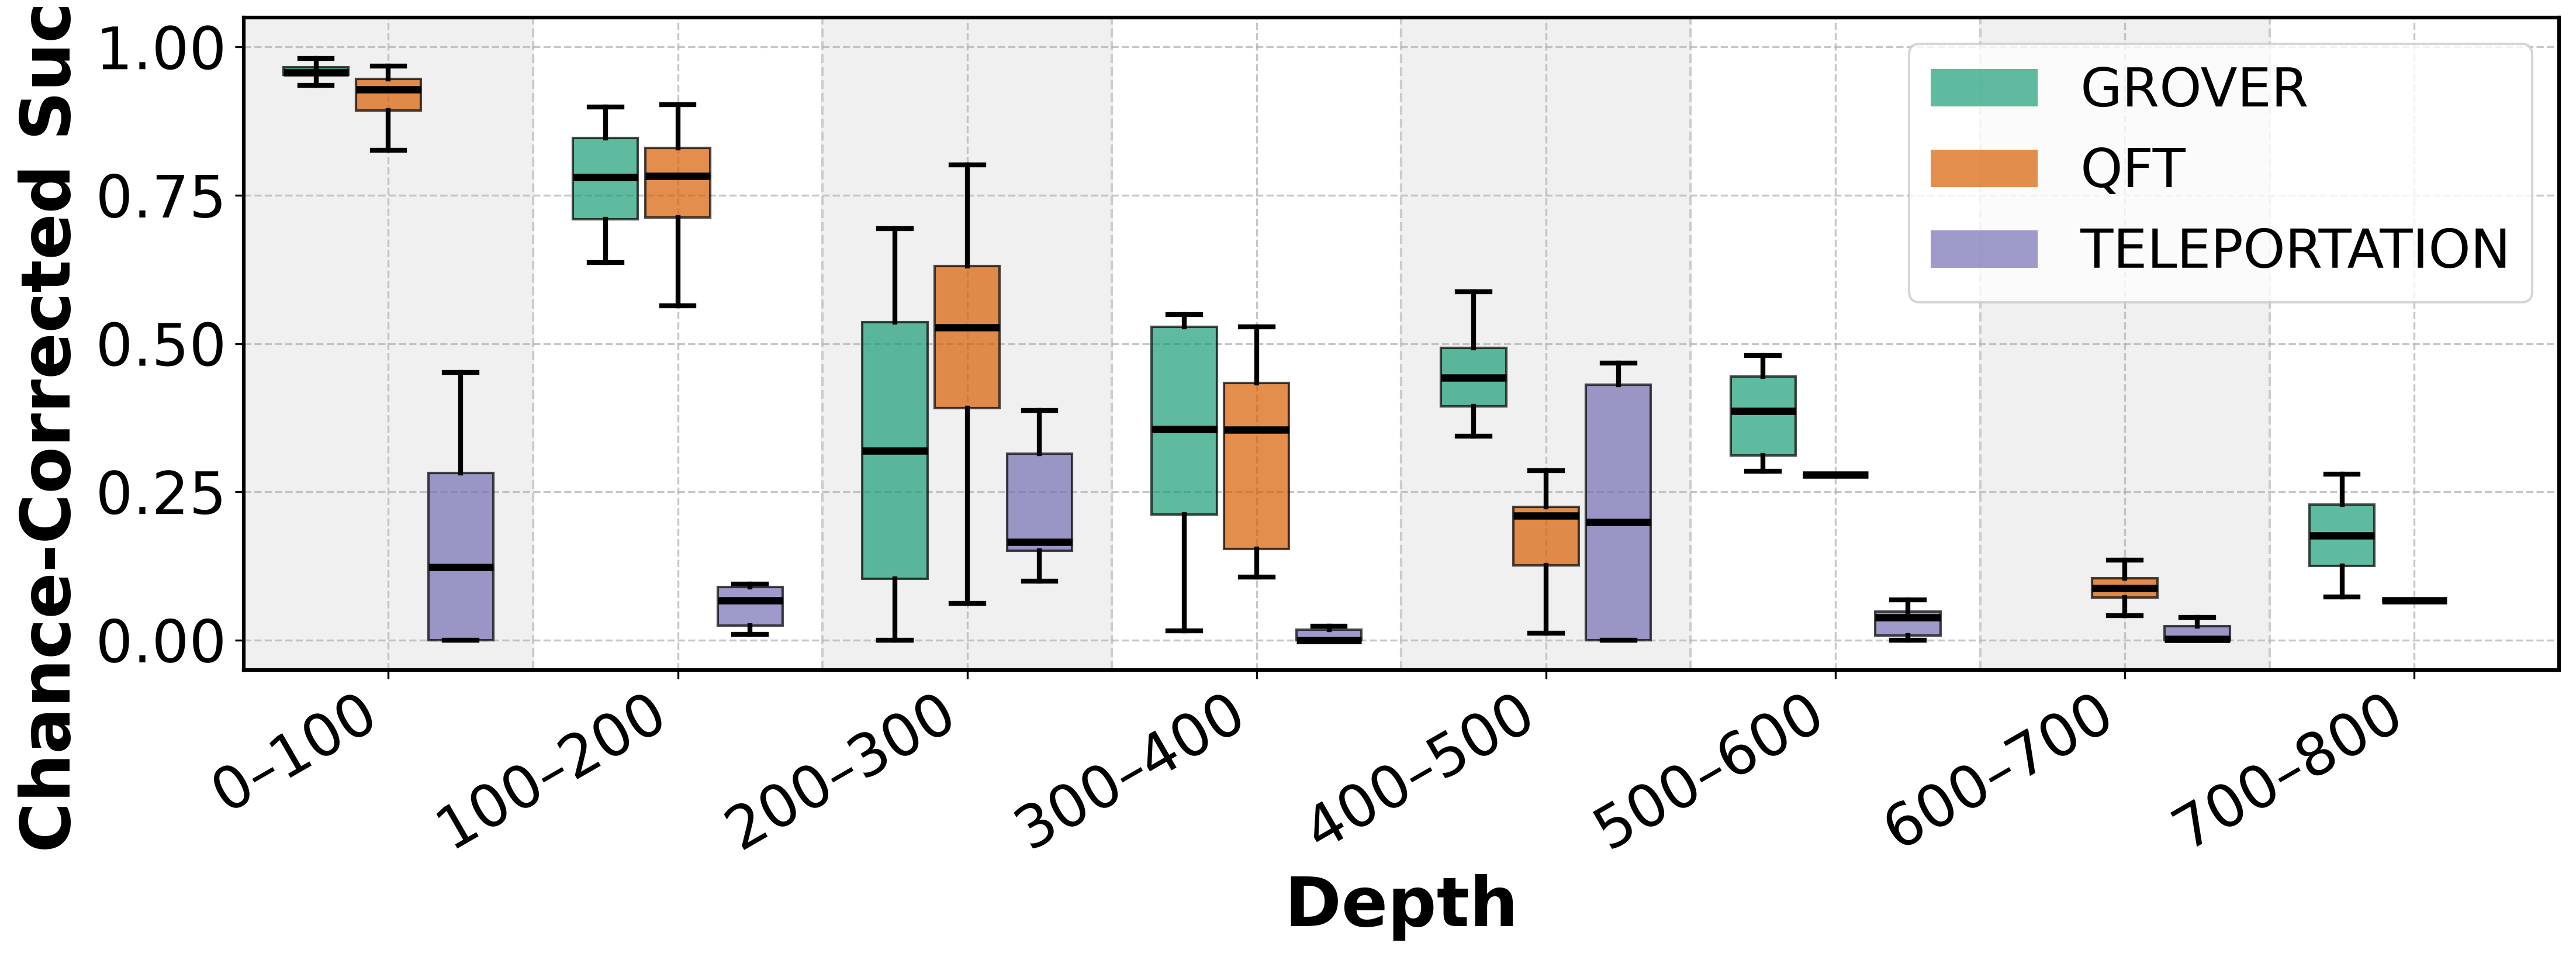
\includegraphics[width=\columnwidth]{plots/2_combined_chance_corrected_comparison_depth_ibm.png}
  \caption{Chance-corrected success vs.\ depth (binned, 100~gates) for Grover, QFT, and vTP across all optimization levels (IBM backends).}
  \label{fig:combined_depth_chance_corrected_ibm}
\end{figure}

The qualitative pattern from the original depth analysis is preserved under chance-corrected success: both Grover and QFT retain high values below 100--200~gates (medians above~$0.75$) and degrade sharply beyond 200~gates, while depth alone remains an imperfect predictor --- the same non-monotonicity previously attributed to multi-marked Grover configurations (M4-4) persists, since chance-corrected success, unlike raw success rate, is a per-configuration rescaling and does not remove that structural dependency. Teleportation's chance-corrected success is markedly lower than either Grover's or QFT's at every depth bin below 500~gates, consistent with the provider-dependent, near-chance IBM performance identified in Section~\ref{subsec:dsr_qubits}.

\subsection{Effect of optimization level on QFT}
\label{subsec:opt_level}

Figure~\ref{fig:qft_heatmap_chance_corrected} displays the median chance-corrected success of QFT executions by qubit count and optimization level.

\begin{figure}[ht!]
  \centering
  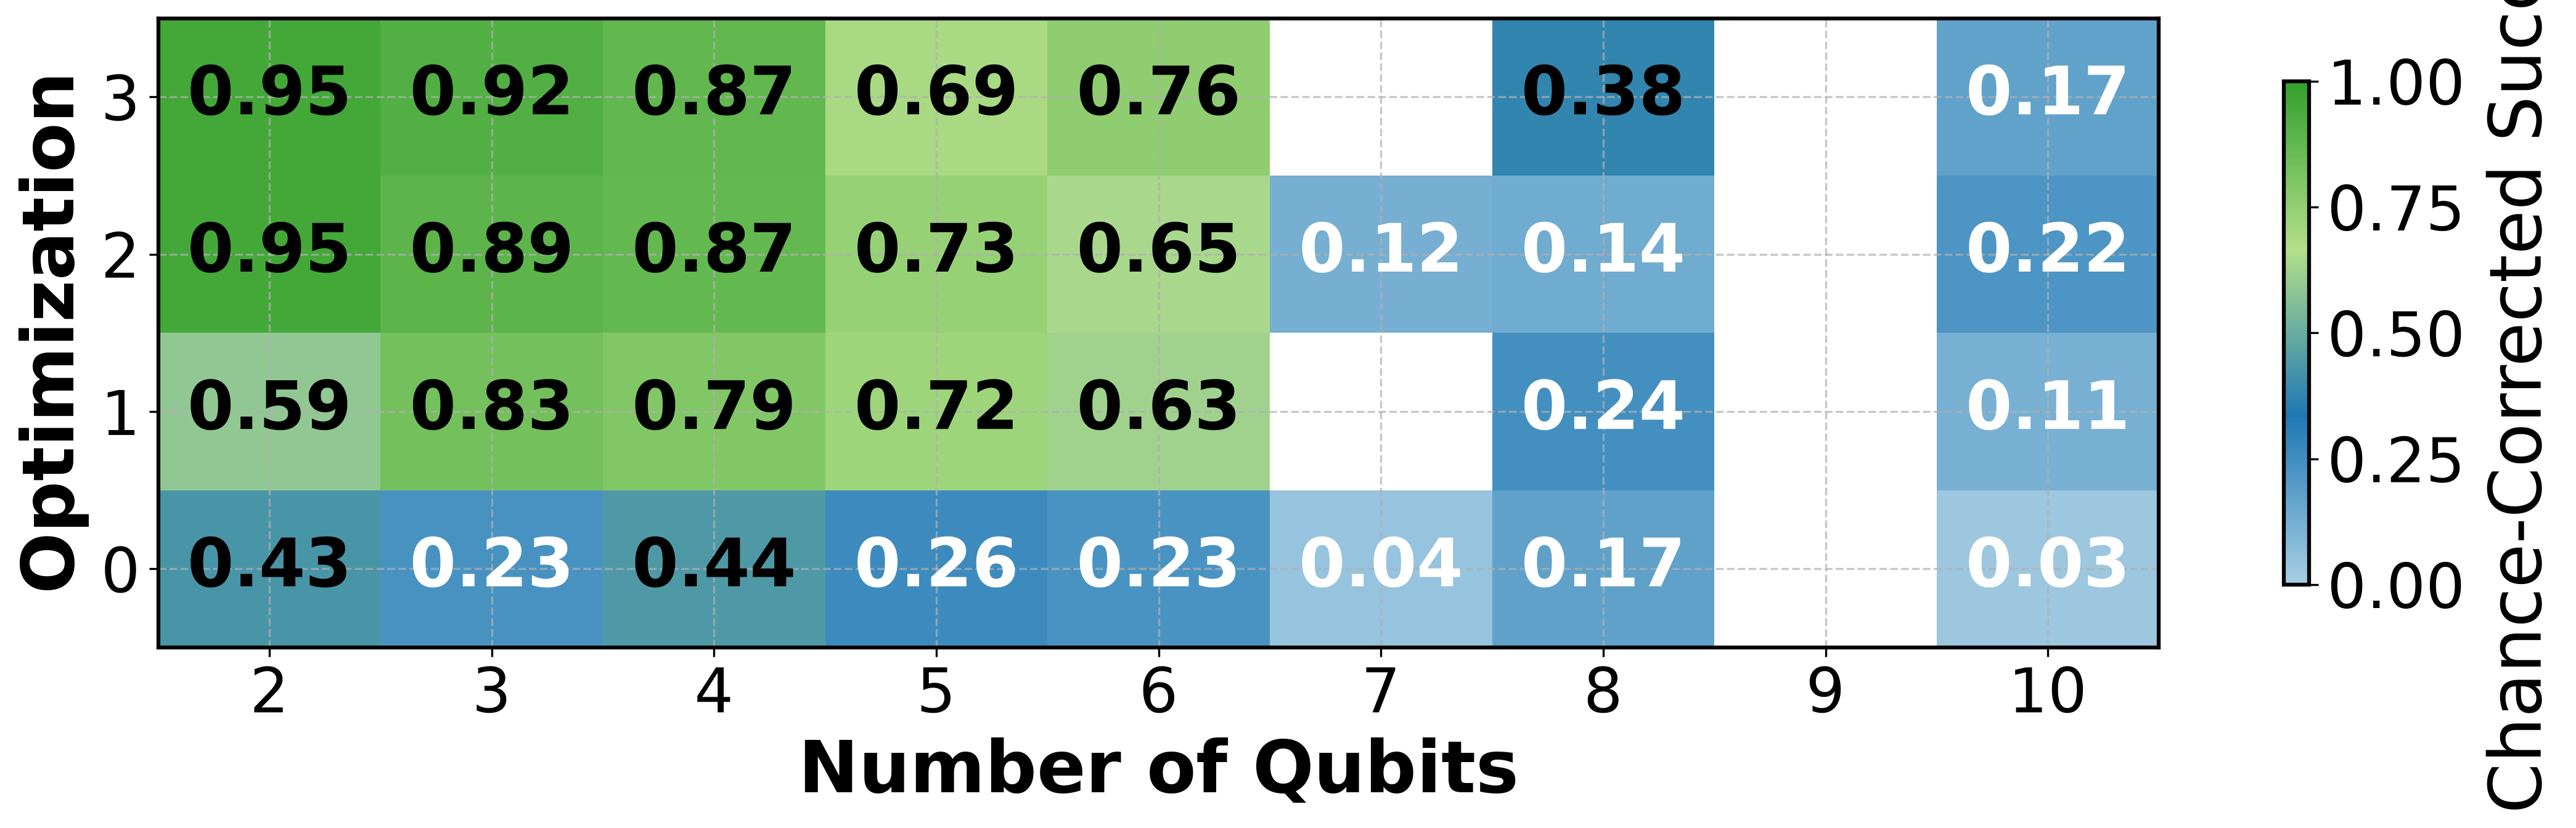
\includegraphics[width=\columnwidth]{plots/2_combined_chance_corrected_qft_heatmap_optimization.png}
  \caption{Heatmap of median chance-corrected success of QFT runs by number of qubits and optimization level (IBM backends).}
  \label{fig:qft_heatmap_chance_corrected}
\end{figure}

The pattern matches the original heatmap's qualitative story: optimization level~0 is low from 2~qubits ($0.43$) and falls further by 5--6~qubits; levels~2--3 remain comparable to each other and substantially better than levels~0--1, with chance-corrected success above~$0.85$ up to 4~qubits at level~3. Level~3 retains a non-trivial value at 8~qubits ($0.38$) and 10~qubits ($0.17$), consistent with the slower degradation of QFT relative to Grover reported throughout this section.


% =============================================================================
% BLOCK 7 -- REPLACES main.tex lines 467-538 (Section "Comparison with other
% fidelity metrics" and Table~tab:stat_comparison)
% =============================================================================

\subsection{Comparison with full-distribution fidelity metrics}
\label{sec:metric_comparison}

Full HF/TVDF describe agreement over the entire $2^m$-outcome distribution and require simulating (or otherwise obtaining) the ideal histogram; the coarse profile components answer a narrower question --- did the job land in the known-correct set $E$, with the right relative weighting across $E$ --- using only counts and~$E$. We first verify where the two agree, then report the recomputed cross-provider comparison using the profile, including the teleportation finding introduced in Section~\ref{subsec:dsr_qubits}.

\begin{figure}[ht!]
  \centering
  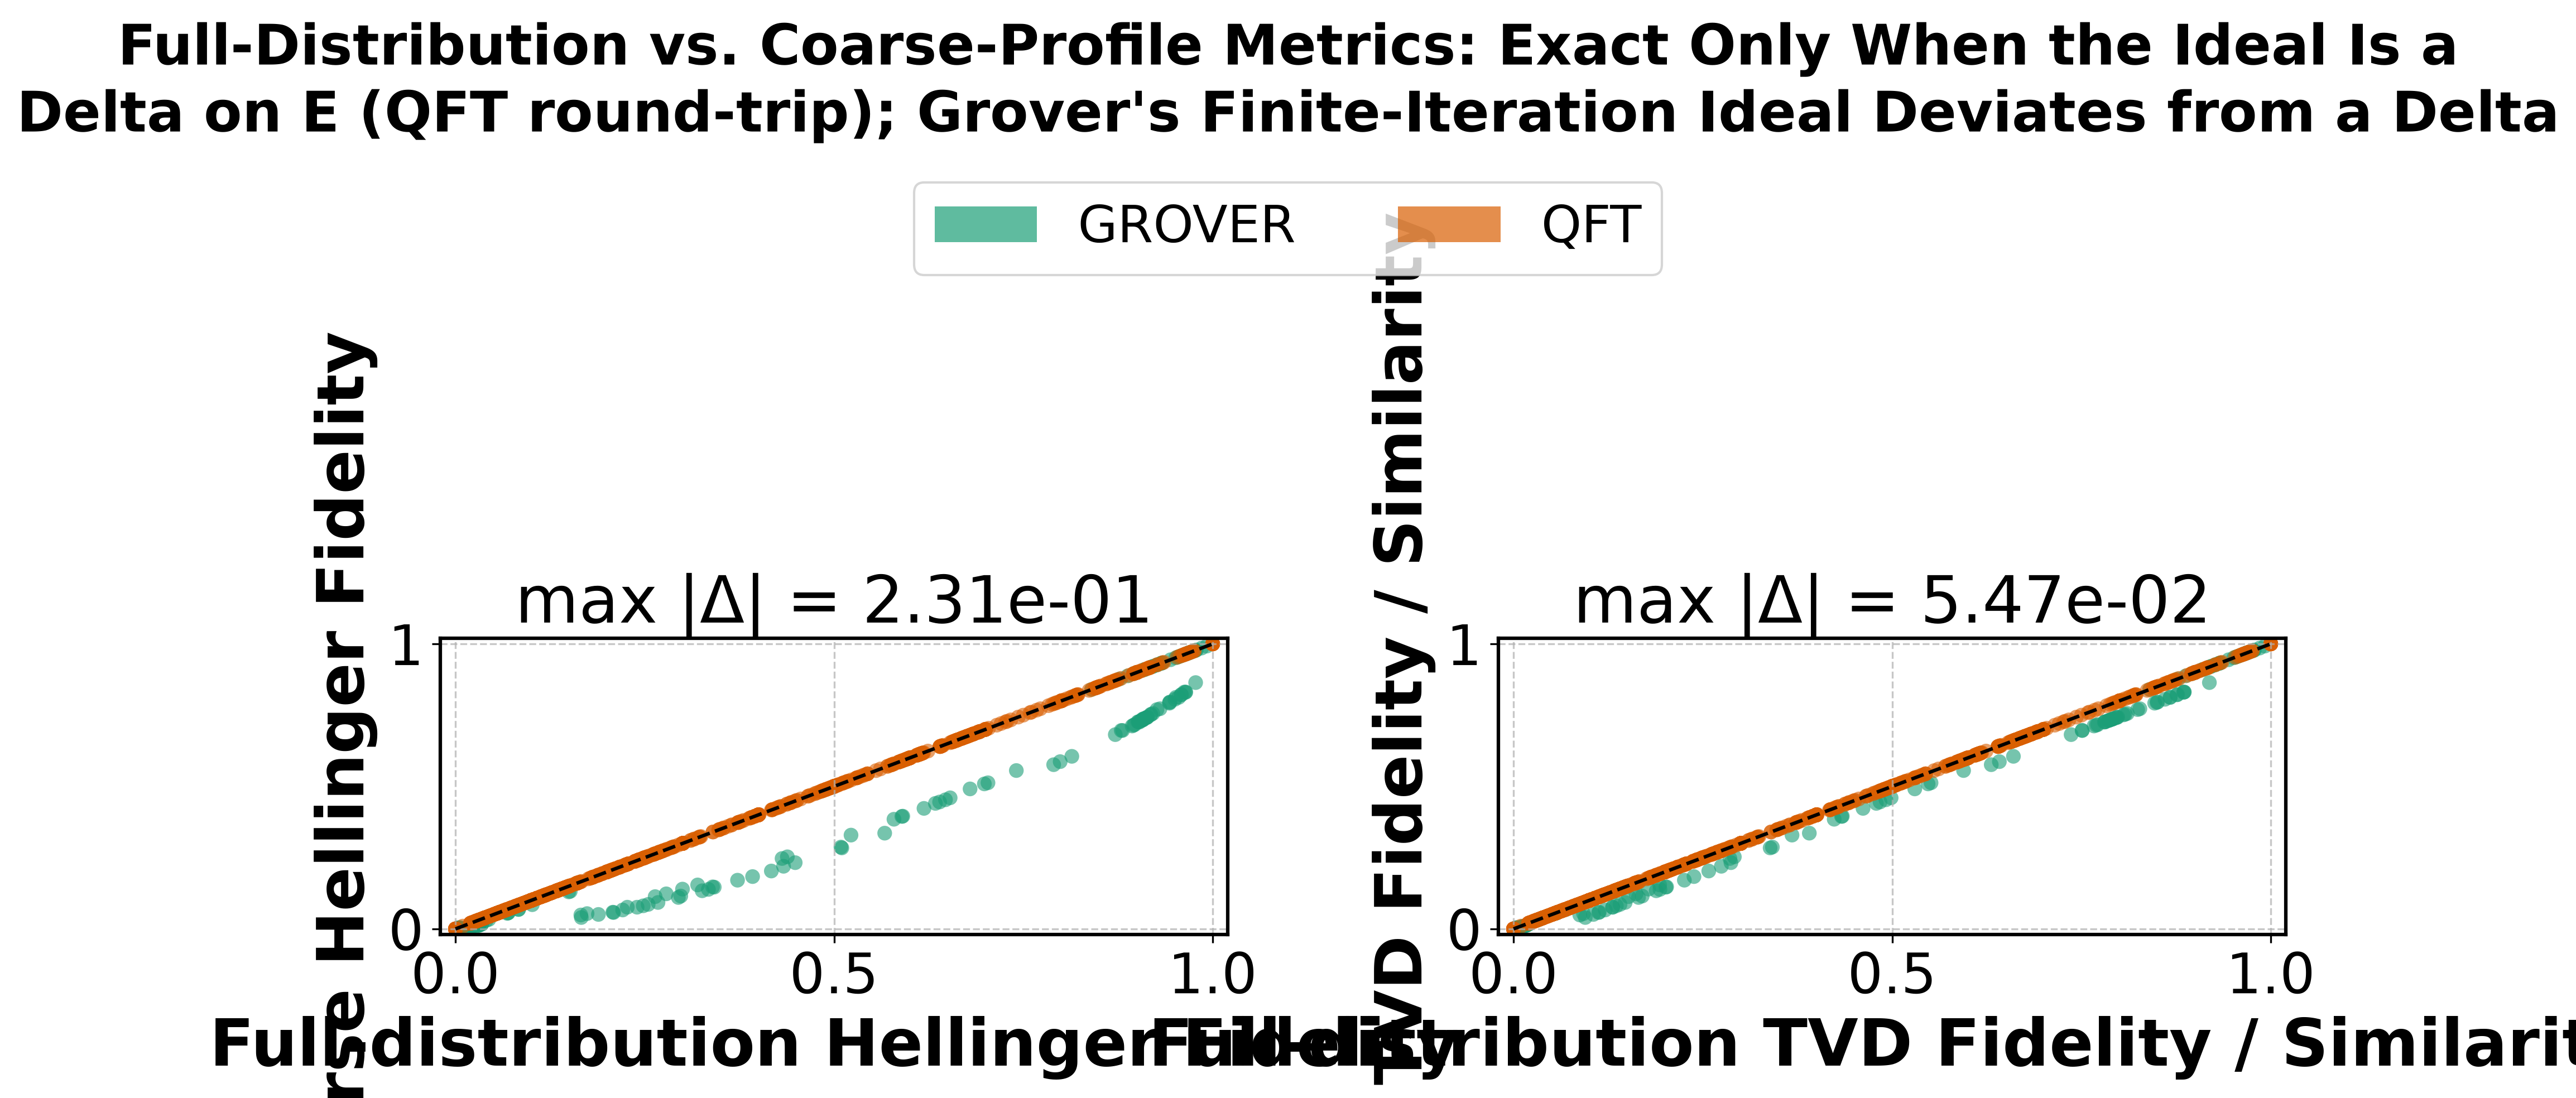
\includegraphics[width=\columnwidth]{plots/2_full_vs_coarse_comparison.png}
  \caption{Full-distribution Hellinger fidelity/TVD fidelity vs.\ their coarse-profile equivalents, for $K=1$ configurations (single-marked Grover, QFT round-trip). Points on the identity line indicate exact agreement.}
  \label{fig:full_vs_coarse}
\end{figure}

As anticipated in Section~\ref{sec:dsr}, Figure~\ref{fig:full_vs_coarse} shows QFT round-trip points falling exactly on the identity line (max deviation $5.5\times10^{-3}$ in TVD fidelity), because its true ideal is an exact delta on $E$. Grover deviates measurably (max deviation $0.23$ in Hellinger fidelity, $0.05$ in TVD fidelity) at high success rates, because Grover's true statevector ideal at a finite iteration count retains residual amplitude outside $E$ (e.g., theoretical success below~$1$ for several configurations, such as $0.9995$ for the single-marked 10-qubit case). This confirms the coarse profile answers "did we get the right answer," a related but distinct question from "did we reproduce the exact ideal state," which only the full-distribution comparison answers.

For multi-answer ($K>1$) configurations, the coarse similarity components can diverge meaningfully from raw success rate whenever the observed success mass is unevenly split across $E$ (Figure~\ref{fig:multi_answer_divergence}); for example, configuration PV4-P8 ($K=8$ QFT period peaks) shows a mean success rate of~$0.92$ but coarse TVD similarity of only~$0.63$, since the coarse components additionally penalize unequal weighting across the expected peaks, not just total mass on $E$.

\begin{figure}[ht!]
  \centering
  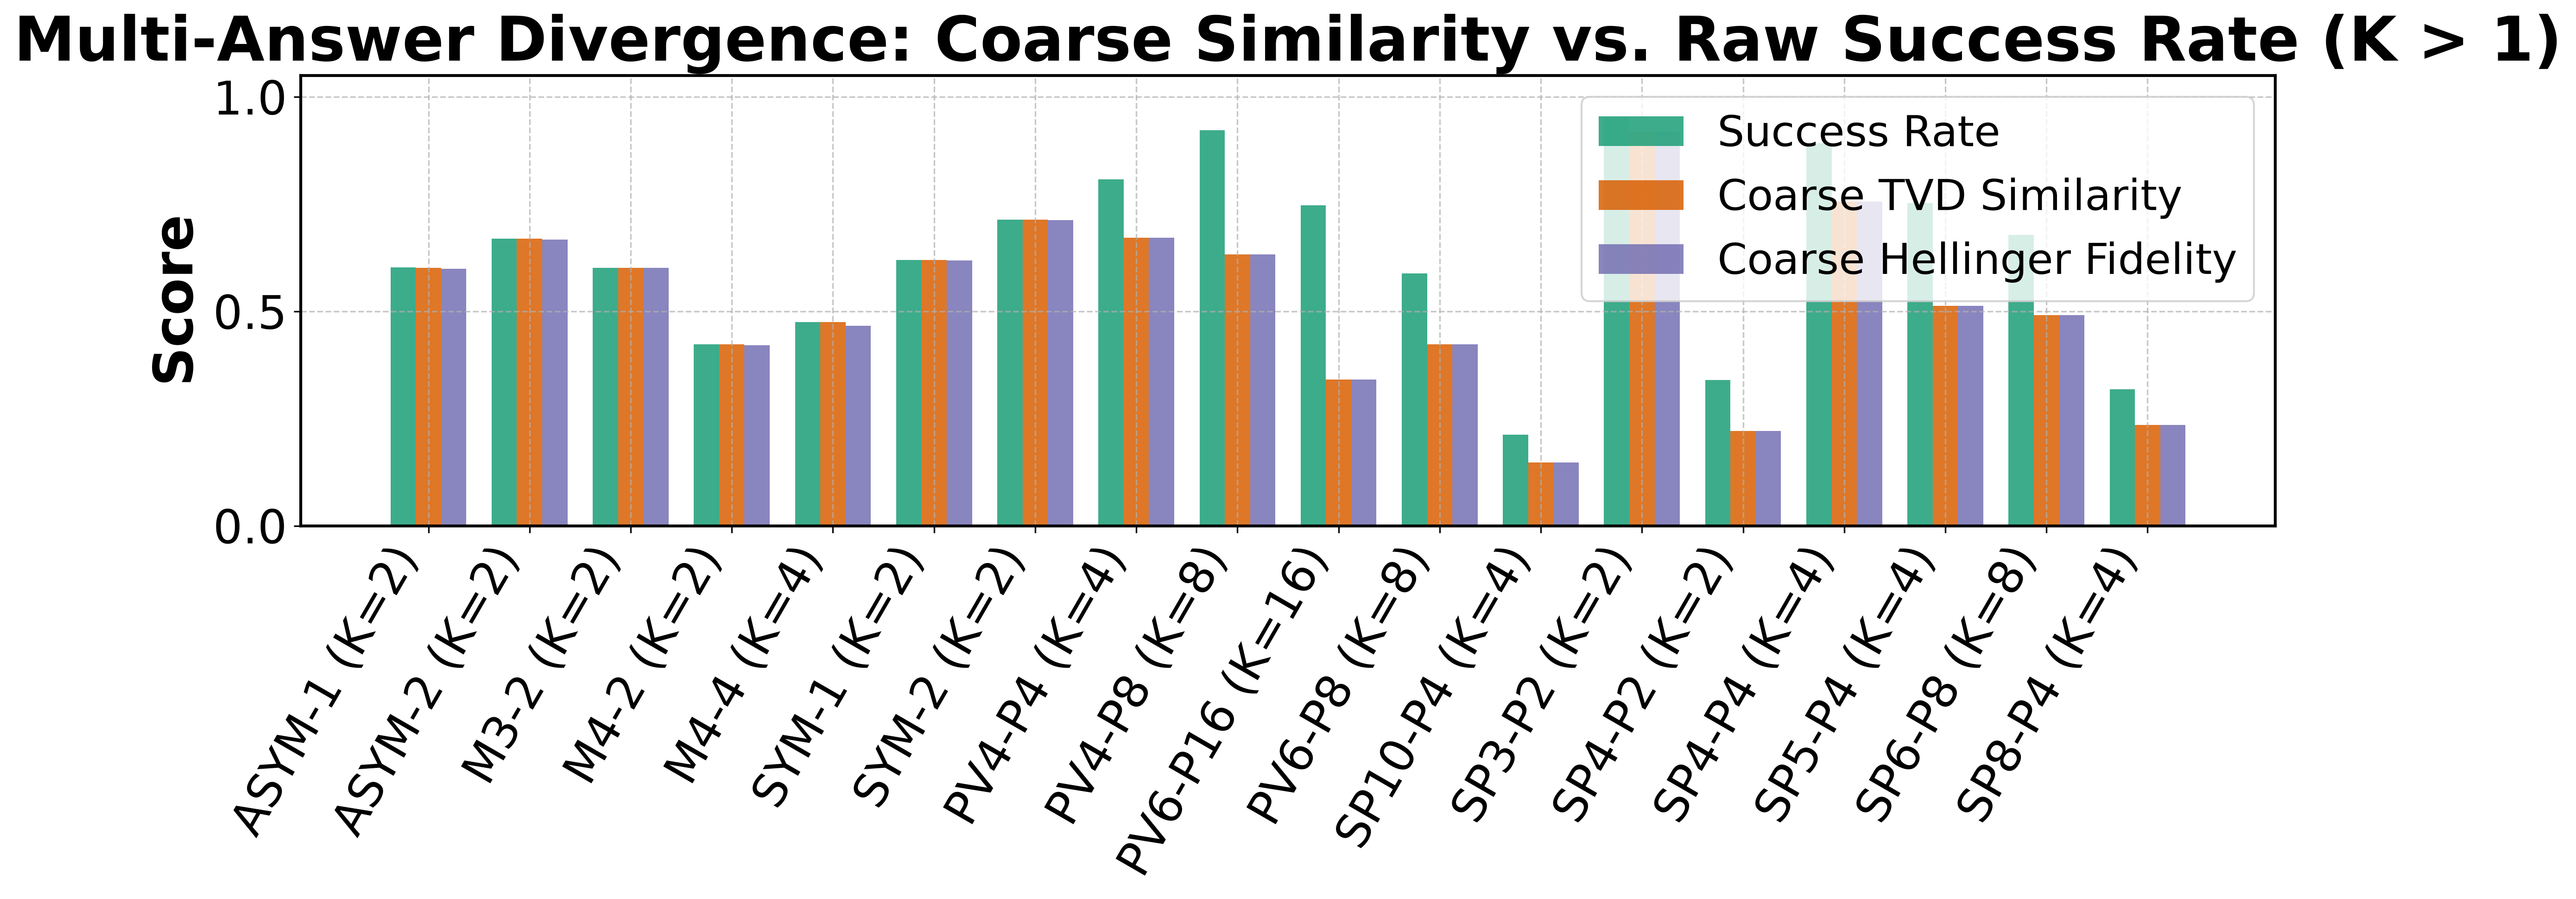
\includegraphics[width=\columnwidth]{plots/2_multi_answer_divergence.png}
  \caption{Mean success rate vs.\ coarse TVD similarity/Hellinger fidelity for $K>1$ Grover and QFT configurations, illustrating divergence when success mass is unevenly split across expected outcomes.}
  \label{fig:multi_answer_divergence}
\end{figure}

\textbf{Grover and QFT: the Rigetti-degrades-earlier narrative is confirmed under the profile.} Table~\ref{tab:profile_provider} (Section~\ref{subsec:dsr_qubits}) shows IBM's chance-corrected success exceeds Rigetti's at every matched qubit count with large effect sizes ($\delta \geq +0.88$) and $p<0.005$ in every group except one underpowered QFT 5-qubit case. This reproduces the qualitative finding of our earlier Michelson-only analysis, but the specific numbers differ: the profile's chance baseline correction and coarse-target restriction to~$E$ replace the earlier full-HF/TVDF "background overlap $\approx 0.25$" framing entirely, so no specific number from the original per-qubit DSR/HF/TVDF comparison table (removed by this revision, superseded by Table~\ref{tab:profile_provider}) should be reused.

\textbf{Teleportation: a new result invisible to the peak-contrast score.} Reevaluating vTP with the profile (previously excluded from cross-metric comparison because Michelson DSR collapsed to~$0$ by 2~payload qubits) reveals a direction \emph{opposite} to Grover/QFT: IBM's chance-corrected success is lower than Rigetti's at every payload size, significant at payloads~3--4 ($p<0.0001$, Cliff's~$\delta \approx -0.8$ favoring Rigetti), while the legacy Michelson score reports $0.000$ on both providers at payloads~2 and~4 --- exactly the T1-bias failure mode described in Section~\ref{sec:michelson-layer}, now demonstrated empirically rather than only theoretically. Because $K=1$ throughout vTP, the coarse TVD similarity and Hellinger fidelity columns equal chance-corrected success up to the chance-baseline rescaling and add no independent signal here; the chance-corrected success component alone is what recovers the provider difference.


% =============================================================================
% BLOCK 8 -- REPLACES main.tex lines 543-552 (Discussion body, keep section
% heading and \textbf{Usability}/\textbf{Applicability} paragraph headers)
% =============================================================================

\textbf{Usability.} The DSR profile is not intended to replace or compete with full-distribution fidelity metrics on their own terms (Section~\ref{sec:inverse-circuit}); its objective is a lightweight, histogram-free complement for the specific, common case of known-answer tasks, where it can be computed at qubit counts beyond what full-distribution simulation supports at all (Section~\ref{sec:broad-ideal}).

\textbf{Applicability.} As with our earlier formulation, the profile is designed for algorithms in which the developer can specify a well-defined expected-outcome set~$E$ (search algorithms, basis-transformation algorithms, state-preparation/transmission protocols). It remains inapplicable to algorithms whose ideal output is a broad probability distribution without a discrete set of dominant states (e.g., variational algorithms); for those, and for any circuit lacking a task-native target, full-distribution HF/TVDF --- optionally via an inverse-circuit construction (Section~\ref{sec:inverse-circuit}) --- remain the appropriate tools.

\textbf{Confounding factors.} Depth alone remains an inadequate predictor of any profile component (Section~\ref{subsec:dsr_depth}), for the same reason identified in our earlier analysis: different circuit configurations (e.g., single- vs.\ multi-marked Grover) map to overlapping depths while degrading very differently. This confound is independent of which component --- chance-corrected success or the original peak-contrast score --- is used as the dependent variable.

\textbf{Threshold behavior, addressed.} Reviewer feedback on our earlier formulation noted that reported values (e.g., $0.51$, $0.28$, $0.11$) did not match a strict threshold (all-high or all-low) interpretation. The profile does not claim threshold behavior for any of its four components; chance-corrected success and the coarse-similarity components are designed to degrade continuously with hardware noise, matching the intermediate values observed throughout Section~\ref{sec:results}. The peak-contrast (Michelson) layer is the only component in this family for which an early, sharper transition was previously observed, and we now report it strictly as an optional layer with a documented failure mode (Section~\ref{sec:michelson-layer}), rather than as the primary evaluation result.

\textbf{Validity considerations.} The same three factors identified in our earlier study continue to apply: sampling uncertainty at low shot counts, correctness of the target set~$E$ itself, and backend calibration drift between jobs. We add a fourth: because the profile's chance baseline $b=K/2^m$ depends on both~$K$ and the measured-qubit count~$m$, values from different $(K, m)$ configurations are only directly comparable via chance-corrected success, not raw success rate; comparisons that mix configurations with different $K$ or $m$ (as in the multi-answer divergence analysis, Figure~\ref{fig:multi_answer_divergence}) should use chance-corrected success or the coarse-similarity components, not success rate alone.


% =============================================================================
% BLOCK 9 -- REPLACES main.tex lines 557-563 (Conclusion body)
% =============================================================================

In this paper, we introduce the DSR evaluation profile, a histogram-free evaluation methodology for the output of quantum algorithms whose correct answers form a known set. Rather than a single new formula, the profile reports four complementary components --- Success Rate, Chance-Corrected Success, Coarse TVD Similarity, and Coarse Hellinger Fidelity --- computed from measurement counts and the expected-outcome set alone, with the original Michelson-contrast score retained as an optional fifth peak-contrast layer motivated by a documented T1-bias failure mode.

To empirically evaluate the profile, we recompute it on 1{,}283 quantum jobs across two providers (IBM Quantum and Rigetti via AWS), spanning Grover's search, the Quantum Fourier Transform, and a teleportation variant, and add a new broad-ideal experiment (multi-marked Grover up to 40~qubits) demonstrating that the profile computes in constant time regardless of qubit count, at scales where full-distribution comparison is not merely slow but requires more memory than exists on any single machine. The recomputed results confirm that Rigetti's Ankaa-3/Forte-1 devices degrade earlier than IBM's Heron~R2 processors on Grover and QFT, and reveal a new, direction-reversed finding for teleportation --- IBM underperforms Rigetti at larger payload sizes --- that the original Michelson-only analysis could not surface, since the peak-contrast score collapses to zero on both providers in exactly that regime. We conclude that the chance-corrected and coarse-similarity components of the profile, not the original peak-contrast score, should serve as the primary indicators of known-answer quantum task success, with the peak-contrast layer retained as a secondary diagnostic.

In future work, we plan to create automated benchmarking pipelines for continuous monitoring of the DSR profile on different quantum providers, to extend the broad-ideal experiment to real QPU execution at qubit counts beyond the classical simulation wall (this paper's broad-ideal results at $n \geq 26$ use representative synthetic counts, not real hardware, since obtaining real counts at that scale requires QPU access beyond the scope of this study), and to benchmark hardware-level gate fidelities against the profile's chance-corrected success component to determine whether it can serve as a lightweight proxy for circuit-level quality characterization.


% =============================================================================
% BLOCK 10 -- FIGURE-RENAMING CHECKLIST
% =============================================================================
% Old figure (main.tex)                              | New figure (this delta)                                          | Status
% ---------------------------------------------------|-------------------------------------------------------------------|------------------------------------
% fig:dsr_variants  (1_grover_dsr_variants_qubits)    | UNCHANGED, retained under Section~\ref{sec:michelson-layer}       | keep as-is
% fig:combined_qubits_ibm (1_combined_dsr_comparison_ibm)      | fig:grover_profile_ibm + fig:qft_profile_ibm (2_*_dsr_profile_comparison_ibm.png)  | superseded, both algorithms now split out
% fig:combined_qubits_aws (1_combined_dsr_comparison_aws)      | fig:grover_profile_aws + fig:qft_profile_aws (2_*_dsr_profile_comparison_aws.png)  | superseded
% fig:combined_depth_ibm (1_combined_dsr_comparison_depth_ibm) | fig:combined_depth_chance_corrected_ibm (2_combined_chance_corrected_comparison_depth_ibm.png) | superseded (Michelson version kept in repo, not cited)
% fig:combined_depth_aws (1_combined_dsr_comparison_depth_aws) | (2_combined_chance_corrected_comparison_depth_aws.png; not cited in text -- optional addition) | generated, available if needed
% fig:qft_heatmap (1_combined_dsr_qft_heatmap_optimization)    | fig:qft_heatmap_chance_corrected (2_combined_chance_corrected_qft_heatmap_optimization.png) | superseded
% fig:grover_metric_comparison (1_grover_metric_comparison_ibm)| fig:full_vs_coarse + fig:multi_answer_divergence (2_full_vs_coarse_comparison.png, 2_multi_answer_divergence.png) | replaced with profile-appropriate comparisons
% fig:grover_metric_comparison_aws (1_grover_metric_comparison_aws) | superseded by Table~\ref{tab:profile_provider}                | table replaces per-algorithm HF/TVDF comparison plot
% tab:stat_comparison                                  | Table~\ref{tab:profile_provider} (this delta)                     | replaced, new numbers, narrower scope (chance-corrected success only, both algorithms combined)
% (none)                                               | fig:2_grover_success_uncertainty_summary, fig:2_qft_success_uncertainty_summary (generated, not cited -- optional addition for a revision round emphasizing shot-noise uncertainty) | generated, available if needed
% (none)                                               | Section~\ref{sec:broad-ideal} scaling figure: 3_broad_ideal_scaling.png | new, cite in Section~\ref{sec:broad-ideal} if a figure is desired there (currently described in prose only)


% =============================================================================
% REPRODUCIBILITY CHECKLIST
% =============================================================================
% 1. Raw data: unchanged QPU/simulator result JSONs under qward/examples/papers/
%    (same files as the original submission; no new hardware jobs were run for
%    the Grover/QFT/vTP recomputation).
% 2. Enrichment (adds success_rate, chance_baseline, chance_corrected_success,
%    coarse_tvd, coarse_tvd_similarity, coarse_hellinger_distance,
%    coarse_hellinger_fidelity, and refreshes dsr_michelson/peak_mismatch to
%    each individual_results entry, in place):
%      PYTHONPATH=. uv run python qward/examples/papers/enrich_dsr_profile.py --dataset all
% 3. Rebuild the unified CSV (adds the same profile columns; computes the
%    profile directly for teleportation rows, which have no enrichment JSON
%    step):
%      PYTHONPATH=. uv run python qward/examples/papers/build_csv_from_json.py
%    Output: qward/examples/papers/DSR_result.csv (1,283 rows: 248 Grover,
%    239 QFT, 796 Teleportation). The 2-row increase in Grover relative to
%    the original submission's 1,281 (246 Grover) is a new raw data file
%    (grover/data/qpu/raw/S2-1_IBM_ibm_fez_20260617_105053.json, 2-qubit
%    single-marked Grover, optimization levels 2 and 3) added after the
%    original submission -- unrelated to the profile recomputation.
% 4. Regenerate profile figures (Block 6 figures 2_*_dsr_profile_comparison_*,
%    2_multi_answer_divergence, 2_full_vs_coarse_comparison,
%    2_*_success_uncertainty_summary):
%      PYTHONPATH=. uv run python qward/examples/papers/dsr_profile_visualization.py
% 5. Regenerate depth/heatmap figures, both legacy Michelson (unchanged
%    filenames) and new chance-corrected-success counterparts
%    (2_combined_chance_corrected_comparison_depth_*, 2_combined_chance_
%    corrected_qft_heatmap_optimization), plus all other unchanged plots in
%    this script:
%      PYTHONPATH=. uv run python qward/examples/papers/differential_success_rate_analysis.py
% 6. Statistics for Table~\ref{tab:profile_provider} and the profile-internal
%    comparison referenced in Section~\ref{sec:metric_comparison}:
%      PYTHONPATH=. uv run python qward/examples/papers/statistical_comparison_profile.py
%    Output: statistical_comparison_profile_internal.csv,
%    statistical_comparison_profile_provider.csv. Teleportation provider
%    numbers quoted in Blocks 1/6/7 are computed ad hoc from DSR_result.csv
%    (grouped by num_qubits=payload size, provider inferred from backend_name)
%    since statistical_comparison_profile.py's provider analysis currently
%    covers Grover/QFT only; extending it to teleportation is a follow-up
%    documented in narrative_assessment.md.
% 7. Broad-ideal experiment (Section~\ref{sec:broad-ideal}):
%      PYTHONPATH=. uv run python qward/examples/papers/broad_ideal_experiment.py
%    Output: broad_ideal_experiment_results.json,
%    broad_ideal_experiment_results.md, plots/3_broad_ideal_scaling.png.
% 8. Narrative gate memo (empirical-story confirmation performed BEFORE
%    drafting this delta, as required by the revision plan):
%    qward/examples/papers/narrative_assessment.md.
% 9. All numeric claims in Blocks 1, 6, and 7 above were read directly from
%    the CSV outputs of steps 3, 6, and 7; none are carried over from the
%    original (Michelson-only, full-HF/TVDF) submission's tables.
